\documentclass[authordate, reflection]{jote-new-article}

\usepackage{caption}

\usepackage{tabularx}

\usepackage{graphicx}

\usepackage{hyperref}

\usepackage[backend=biber,style=apa]{biblatex}

\addbibresource{bibliography.bib}

\jotetitle{Adopt a cultural-historical perspective to adapt misinformation interventions: Reflecting on Harjani et al.}
\keywordsabstract{misinformation, inoculation theory, intervention mapping, cultural adaptation, cultural-historical theory}
\abstracttext{Harjani et al. (2023) conducted a gamified inoculation intervention against misinformation in rural India. Despite the ingenuity of the intervention design, the study revealed no significant effects on participants' ability to detect misinformation, highlighting cultural and digital barriers to effective intervention. We argue from a cultural-historical perspective that conceptual development stages, influenced by formal education, play a crucial role in the success of interventions. From a practical perspective, we propose a possible guideline following the adaptation recommendations proposed by the theory of Intervention Mapping. Our reflection provides a deeper understanding of why traditional inoculation methods may prove ineffective in more rural and less literate regions and suggests pathways for developing more culturally attuned and effective interventions.}
\runningauthor{Panizza et al.}
\jname{Journal of Trial \& Error}
\jyear{2025}
\paperdoi{10.36850/415c-479a}
\paperreceived{August 7, 2024}
\author[1]{\mbox{Folco Panizza\orcid{0000-0001-5178-5926}}}
\affil[1]{IMT School for Advanced Studies, Lucca, Italy}
\corremail{\href{mailto:panizzafolco@gmail.com}{panizzafolco@gmail.com}}
\corraddress{IMT School for Advanced Studies Lucca}
\runningauthor{Panizza et al.}
\author[2]{\mbox{Thomas Camminga\orcid{0000-0002-8804-4432}}}
\affil[2]{Radboud University, Nijmegen, the Netherlands}
\author[2]{\mbox{Stefan Gaillard\orcid{0000-0003-1956-7325}}}
\author[3]{\mbox{David Joachim Grüning\orcid{0000-0002-9274-5477}}}
\affil[3]{Heidelberg University, Heidelberg, Germany}
\paperaccepted{February 5, 2025}
\paperpublished{March 31, 2025}
\paperpublisheddate{2025-03-31}
\jwebsite{https://journal.trialanderror.org}

\begin{document}
\begin{frontmatter}
  \maketitle
  \begin{abstract}
    \printabstracttext
  \end{abstract}
\end{frontmatter}







	\section{Introduction}



	In the digital age, the spread of misinformation is a major public challenge that requires innovative interventions to combat its spread and influence. Digital interventions, which take advantage of advanced technologies and the wide reach of the internet, have emerged as important tools for disseminating accurate information, countering false narratives, and fostering critical thinking among the public (e.g. Horta Ribeiro et al., 2023; Katsaros et al., 2024; Kiili et al., 2024; Lin et al., 2024; Matias, 2019). One type of novel application in the field of digital counter-misinformation campaigns is the online, gamified version of inoculation interventions originally developed in social psychology (McGuire, 1961). Analogous to its medical counterpart, an inoculation involves exposing individuals to a diluted form of misinformation (e.g. van der Linden, 2023). The goal of inoculation interventions is to foster cognitive resistance to misinformation by equipping individuals with the skills to critically evaluate and question the veracity of information they encounter online. However, to date, inoculation interventions have almost exclusively been conducted in populations from continental Europe, the United Kingdom, and North America (Basol et al., 2020; Roozenbeek et al., 2022). In contrast to the results of studies conducted in Western contexts, Harjani and colleagues (2023) found no evidence for the effectiveness of an adapted version of a commonly used inoculation game. The present reflection article aims to expand on the explanations of Harjani et al. (2023) for why the inoculation game failed to show any effects in a large sample of Indian participants. In doing so, we focus on a practical solution via Intervention Mapping and a theoretical model that can explain differences in intervention effectiveness across cultures, specifically cultures with high and low literacy rates (Ghai, 2021).



	\section{Summary of Harjani et al.'s Study}



	The concept of inoculation theory, originally from immunology, has been adapted to digital interventions to combat misinformation. Like its medical counterpart, where exposure to a weakened virus builds immunity, psychological inoculation involves exposing individuals to diluted misinformation to foster cognitive resistance. By equipping individuals with critical evaluation skills, these strategies aim to enhance resilience against the spread of misinformation online. Such interventions have been tested across various iterations (Basol et al., 2020; Roozenbeek et al., 2022) and contexts (Iyengar et al., 2022; Ma et al., 2023).



	To address the narrow demographic focus in prior research (Henrich et al., 2010), Harjani et al. (2023) evaluated a gamified inoculation intervention in rural India. Their randomized control trial (\emph{n} = 757) compared control and treatment groups over time using “Join this Group,” a specifically developed inoculation game. Participants rated the reliability of WhatsApp conversations containing misinformation, their confidence in their reliability rating, and their willingness to share the information. The results showed no significant effects of the intervention on participants' reliability ratings, confidence, or sharing behavior.



	\section{Explanations by the Authors: Digital and Cultural Barriers}



	Harjani et al. discuss several limitations in the experimental design and data collection that may have contributed to the ineffectiveness of the inoculation game. Specifically, these are the lack of digital literacy and familiarity with digital tools among the sample surveyed, and the use of tools developed in other social and cultural contexts.



	\subsection{Digital Barriers}



	Despite several disciplines and theoretical frameworks that have tried to encompass it, digital literacy remains an elusive concept that is difficult to define (Guess \& Munger, 2022). Broadly speaking, digital literacy refers to the ability to reliably assess information in digital environments. Digital literacy requires a good command of digital devices: One potential issue with the study was indeed the use of digital devices in contexts where digital literacy is expected to be low. As the authors themselves acknowledge, it is likely that the “game-based intervention was conducted on participants with minimal experience with operating digital devices” (Harjani et al., 2023, pp. 10-11): In the rural areas where the study was conducted, it is estimated that there are 25 digitally literate households for every 100 (Mothkoor \& Mumtaz, 2021).



	Studies on misinformation trying to reach vulnerable populations with low digital literacy are faced with the limitation of how to reach these populations. A brief review of experiments conducted across several countries suggests that researchers are finding several solutions to the problem. Several studies rely on existing polling firms and online recruitment platforms (Arechar et al., 2023; Pereira et al., 2022; Porter et al., 2023), but information about the demographic composition of the samples is either lacking or skewed toward the more educated (Badrinathan \& Chauchard, 2024).\footnote{ One study, conducted in 16 different countries (Arechar et al., 2023), focused on the representativeness of their samples in terms of age and gender, attempting to match the demographics of each country. However, the study relied on online worker platforms such as Lucid to recruit participants and therefore reached a largely digitally literate audience. One study targeting COVID-19 misconceptions and reaching large audiences in multiple countries appears to show the effectiveness of fact-checking messages (Porter et al., 2023), but the demographics in many countries appear to be skewed toward the more educated (Badrinathan \& Chauchard, 2024). Another experiment in Brazil, conducted with a polling firm, reports a significant impact of inoculation, but lacks the demographics of the respondents (Pereira et al., 2022).} Another sampling approach is to disseminate online surveys through advertisements on social media (Athey et al., 2023; Garg and Yadav, 2022; Iyengar et al., 2022; Offer-Westort et al., 2024; Porter \& Wood, 2021;). For example, Grag \& Yadav (2022) reached a large sample of respondents in Uttar Pradesh through Facebook ads and found a significant effect of an inoculation intervention. However, 83\% of the sample reached were college graduates, who make up 5\% of the general population in the region. Another issue of ad recruitment relates to the use of English in countries where English is not widely spoken in rural areas (Brown, 2005; Translators without Borders, 2019), or where misinformation is spread through local languages (Saxena \& John, 2021). A third approach is to sample participants through popular direct messaging apps (Bowles et al., 2020; Bowles et al., 2023; Gavin et al., 2022). Despite some improvements, this sampling process has been shown to be susceptible to the same biases towards the better educated as other methods.



	In the experiment that is the subject of this reflection, the authors relied on door-to-door sampling, bypassing the filter of online sampling. However, respondents were provided with smartphones and tablets to complete the survey, devices with which they may have been unfamiliar. Evidence of the negative effect of device unfamiliarity comes from a recent study in Côte d'Ivoire that used tablets to collect responses: The interventions studied failed to reach significance at the 5\% level, and some interventions even appeared to induce increased skepticism about the real news provided (Gottlieb et al., 2022).



	Digital limitations may partly explain the lack of effect of the intervention, as participants may have found it more difficult to understand and respond to the game. However, supplementary analyses including only those participants who correctly entered the game password (a proxy for digital literacy) did not reveal any significant differences from the full sample. Indeed, digital tools and recruitment methods may not be the sole barrier to overcome; testing the offline success of successful online strategies against misinformation, without any digital support has mostly yielded null results. Experiments conducted in India and Pakistan using printed surveys, and occasionally with minimal audio-visual support, reported either no effect of the misinformation intervention studied (Badrinathan, 2021; Guess et al., 2020), or an effect that was largely driven by participants with higher digital literacy (Ali \& Qazi, 2023). Indeed, this incomplete review suggests a particular pattern: The greater the distance from typical online samples, the less likely it is that the misinformation intervention designed to work online will be effective. Of course, there are a few notable exceptions, each with its own peculiarities. (Amar et al., 2024; Badrinathan et al., 2024). An example is the study by Badrinathan et al. (2024), which successfully reduced support for vigilantism in India and Pakistan. Interestingly, however, rather than exporting an online strategy to spot misinformation, the intervention relied on mimicking traditional mass media communication channels: The intervention was a very credible mock radio broadcast that sounded like a professional news report.



	\subsection{Cultural Barriers}



	 Our interpretation of these results is that the more we move away from highly urbanized and literate samples, the less appropriate online interventions themselves are for countering misinformation (see also Badrinathan \& Chauchard, 2024; Blair et al., 2023; Roozenbeek et al., 2024). In other words, beyond digital boundaries, there are other cultural and social boundaries that compromise the effectiveness of interventions when translating them into another context (Dahdouh-Guebas et al., 2003). One instance of cultural barriers may be that examples used in the intervention originating from the first culture may not apply to the experiences of individuals from the second culture. This perspective may help to explain the gap between the current findings and the effectiveness of the intervention in other countries or even in more urbanized areas of India. Indeed, previous comparisons between urban and rural areas of India have shown how another misinformation intervention (media literacy) was largely effective with a sample of online respondents but failed with a sample of Indians living specifically in rural areas (Guess et al., 2020).



	We thus agree with Harjani et al. (2023) that digital and cultural barriers may indeed be daunting challenges to designing interventions against misinformation in rural populations. In the following sections, still, we offer two perspectives that may contribute to building new interventions for these contexts. First, we outline Vygotsky's cultural-historical perspective, which may provide a deeper understanding of the cultural barriers preventing an effective transfer of interventions from mostly digitally literate to rural populations. After that, we will discuss intervention mapping: a practical protocol for adapting interventions to new communities.



	\section{A Cultural-Historical Perspective}



	While cultural differences likely impede the generalizability of results, we suggest that the underlying reasons for the untranslatability of the results may run deeper. Based on the principles of cultural-historical theory, we theorize that the null findings in the Harjani article may be related to differences in levels of conceptual development. Cultural-historical theory views development not as a gradual maturation of innate psychological processes, but as a hierarchical process where new psychological functions are shaped by cultural influences.\footnote{Note that this conceptualization of development differs from a perspective based on local adaptations, where different forms of thinking are simply adaptations to local circumstances. According to the cultural-historical perspective, different forms of thought hierarchically build upon each other, and formal schooling plays an important role in the transition to the later stages.} Vygotsky (1934/2012) and later Toomela (2020a, 2020b), distinguished stages in conceptual development based on differences in the use of signs in mental operations. We will briefly outline this theory and will argue how it could make sense of the null result of the Harjani et al. paper.\footnote{It is important to note that one can disagree with Vygotsky's philosophy of perception and epistemology (as indeed some authors of this article do), while at the same time acknowledging the utility of his framework for understanding differences in cognitive and conceptual development across cultural contexts.}



	\subsection{Semiotic Mediation}



	Lev Vygotsky (1896-1934), a Russian psychologist, is widely recognized as a prominent historical figure in the field of psychological development. Together with his collaborator Alexander Luria, he focused on how the internalization of cultural tools transforms the relationship between humans and their environment. According to Vygotsky (1934/2012), humans store information in the form of signs. In general, a sign is “a wholistic unit containing an image composed of sensory attributes as one of its parts, and an aspect of the external world as another part, or another image that is associated with that first image” (Toomela, 2020a, p. 155).



	There are two types of signs according to this perspective. First, sensory-based signs are directly connected to a part of the external world. A child sees a brown trunk with leaves, and a mental image (or ‘representation') that represents trees is activated in the mind—the tree is recognized as a tree. Secondly, there are linguistic signs. In this case, a verbal signifier, such as a spoken word (e.g., “tree”), is connected to the mental image which is, in turn, still related to the external world. The link between the verbal signifier and the tree in the real world is thus indirect. Contrasting to natural signs, linguistic signs can be brought in different contexts than their referents. Thus, people can say the word “tree”, and thereby recall an image of a tree, while being in a concrete building.



	Vygotsky's ideas remained relatively unknown outside Russia for the better part of the 20th century, but in recent decades, his ideas have been rediscovered and further developed by scholars (e.g., Alderson-Day \& Fernyhough, 2015; Toomela, 2020a; Valsiner et al., 2017). Cultural neuropsychologist Aaro Toomela (2020a, 2020b) proposed that linguistic signs allow humans to make sense of their environment in different ways. Verbally, the same reality can be described in different or even conflicting ways. By resolving these conflicts, humans can become aware that not all aspects of the world are directly available to the senses. Importantly, some types of knowledge can only be arrived at based on signs with a certain structure. For example, the existence of atoms and the evolution of species cannot be seen, heard, or touched directly, but their existence can be conjectured and tested experimentally in indirect ways. Thus, based on linguistic signs, humans learn to construct abstract knowledge beyond the immediately sensed present.



	\subsection{Stages of Sign Development}



	Vygotsky (1934/2012) suggests that there are different stages in the development of linguistic signs that correspond to different ways of thinking. This theory has been elaborated by Toomela (2020b), and we will rely on his terminology in the following. In the present paper, we discuss two stages (see Table 1) distinguished by both Vygotsky and Toomela that may be crucial to understanding the null result of the target article, namely everyday concepts and logical concepts (or ‘scientific concepts' in Vygotsky's terms).



	\begin{table*}
		\begin{fullwidth}
			\begin{threeparttable}
				\caption{Comparison between everyday concepts and logical concepts}
				\begin{tabularx}{\linewidth}{@{} >{\RaggedRight\arraybackslash}p{11.5em} >{\RaggedRight\arraybackslash}X >{\RaggedRight\arraybackslash}X @{}}
					\toprule   & Everyday concepts & Logical concepts \\

					\midrule Referents & Words refer directly to mental images.  &
					Words may refer hierarchically to other words, and thus only indirectly to sensory experiences. The link to mental images is indirect.
					\\

					Category boundaries &
					Categories have fuzzy boundaries based on perceptual similarities and everyday situations.
					& Categories have strict all-or-none type boundaries. \\

					What can be represented &
					Whole sensory, as well as aspects of the nonsensory world can be represented (but understood in concrete and everyday terms).
					& Coherent and logical understanding of the sensory and nonsensory world.
					\\

					Constraints on thinking & Thinking is bounded by concrete experiences. &
					Abstract problem solving becomes possible, in a purely verbal context. Thought itself can be reflected on, allowing for critical thinking.
					\\

					How are they learned & Primarily by participating in society. &
					Formal schooling, reading. \\

					\midrule Example (evaluation of medical information) & “Smoking is not dangerous. My grandfather has smoked all his life and he is still healthy.”
					& “Smoking increases the probability of lung cancer, as indicated by prospective cohort studies.”
					\\
					\bottomrule


				\end{tabularx}
				\vspace{3pt}
				\emph{Note}. Adapted from Camminga et al. (2024).
			\end{threeparttable}
		\end{fullwidth}
	\end{table*}

	







	Everyday concepts rely on linguistic signs that are directly linked to mental images. Categories signified by words at this stage have fuzzy boundaries, meaning that things can belong to the category in different degrees. Everyday concepts allow us to describe all aspects of the world as perceived by the senses, meaning that every situation that can be observed by humans can be put into words. This includes past and future scenarios, potentially even over long stretches of time and space, as well as fictional stories and myths. However, all knowledge at this stage, even in reference to apparently non-sensory phenomena, such as religious ideas, is understood in concrete, everyday terms (e.g., "Natural phenomena are controlled by spirits with human-like qualities"). In a similar vein, an understanding of mental processes of both other people and oneself can start to develop at this stage, but these are also understood in a concrete sense. For example, ‘knowing' is understood as ‘having seen it with my own eyes.' Due to the possibilities to describe and conceptualize current and future situations, everyday concepts are sufficient for developing agriculture and complex societies. Nevertheless, this stage is still limited because it does not permit a critical evaluation of thought processes through abstract logical analysis, independent of the sensed reality that these thoughts address. This changes in the next stage.



	At the stage of logical concepts, linguistic signs can hierarchically refer to other words. Thus, the relationship to mental images becomes indirect. To refer to the earlier tree example, taxonomy is a logical concept: A child can learn the word “plant,” which first hierarchically refers to trees as well as other types of plants, before referring to mental images that represent specific plant species. At the stage of logical concepts, thought can become increasingly abstract and it becomes possible to reliably establish and justify knowledge about aspects of the world that are not available to the senses. With the possibility of describing language with language it also becomes possible to reflect on thoughts, beliefs, and feelings as abstract mental processes. Justifications of beliefs at this stage can go beyond statements of direct observation, considering more indirect observations. For instance, individuals cannot directly observe some phenomena taking place (e.g. a viral infection) but can consider non-sensory phenomena (e.g. blood samples) to confirm or falsify one's predictions. In addition, it becomes possible to test whether conclusions follow logically from their premises.



	\subsection{The role of education in the acquisition of logical concepts}



	The transition from everyday to logical concepts takes place primarily in formal schooling. This is because abstract concepts, such as those discovered by science, are too remote from direct experiences to be learned through incidental learning (e.g., imitation). The impact of formal education on thought processes is illustrated by a series of experiments by Luria (1976) in Uzbekistan, an agricultural region that was largely illiterate at the time.



	Starting from the 1920s, the Soviet Union introduced literacy programs to teach illiterate farmers basic skills in reading, writing and arithmetic, and bringing the farmers into more theoretical concerns beyond their everyday experiences. Luria's (1976) comparative research on individuals who had received education versus those who had not, provided early evidence for the changes in mentality following formal schooling, as well as clear examples of thought based on everyday concepts as opposed to logical concepts. For example, Luria (1976) presented the farmers with syllogisms such as the following: “Cotton can grow only where it is hot and dry. In England it is cold and damp. Can cotton grow there?” (p. 108). One of the farmers responded as follows: “I don't know. [...]. I've only been in the Kashgar country; I don't know beyond that” (p. 108). The participants of the education programs, in contrast, had little difficulties solving such syllogisms, i.e., to solve problems intra-linguistically. More recently, Toomela et al. (2020a, 2020b, 2023) conducted a series of experiments comparing illiterate individuals from Brazil with literate people from Brazil and Estonia and found that illiterate people relied almost exclusively on everyday concepts. The groups scored very differently on tests of visual analysis, cognitive inhibition, and self-analysis, showing that the mind may change drastically in the transition between everyday to logical concepts (see also Ardila et al., 2010; Ardila \& Roselli, 2007).



	\subsection{Back to the experiment}



	Thus, individuals with different levels of education may rely on drastically different ways of thinking, which are at least in part due to differences in education. This further emphasizes the idea that psychological findings that hold in one group may not apply to another, even within the same culture. Applying these cultural-historical ideas to the target article, it becomes clear that in devising strategies against misinformation, we should consider the type of concepts the target population relies on predominantly. The sample of Harjani et al. (2023) was at least literate, so there is no one-to-one comparison with Luria's example with illiterate farmers. Still, the authors estimate that 74\% of their sample is rural. Rural areas of India are on average less educated than urban areas, as indicated for example by the lower literacy rate (67.8\% compared to 80.90\% in urban areas; Registrar General of India, 2011). Given that logical conceptual thought is acquired predominantly in formal schooling (Toomela, 2020), the individuals in the sample may rely predominantly on everyday concepts.



	The inoculation method itself can be seen to prompt logical conceptual thinking, as it causes individuals to construct knowledge about their own thought processes (e.g., by considering the emotional responses generated by certain content, or by trying to trace back the thought process of malicious agents). We argue that such an intervention may have different effects depending on the degree to which the individuals have relied upon logical concepts prior to the intervention. Even the very nature of misinformation may differ depending on the level of sign development within the reference group, rendering certain strategies not only ineffective but also off the mark. Inoculation strategies to combat misinformation originated in and have been shown to be effective in contexts where logical conceptual thinking is ubiquitous.



	How exactly individuals relying on everyday concepts and logical concepts differ in how they make sense of the material presented in inoculation interventions may be an interesting topic to explore for future research. We propose one way that effects of the intervention may differ for everyday conceptual and logical conceptual thinkers. The acquisition of logical concepts is a drawn-out developmental process, and a single intervention cannot go far in reorganizing conceptual knowledge. Interventions may allow individuals who have learned to think logically conceptually to transfer logical concepts to new contexts. Therefore, inoculation may benefit individuals who have already learned to think logically conceptually in at least some areas, whereas for predominantly everyday conceptual thinkers, the strategy may not transfer so easily, even if it was effective in promoting logical conceptual thought in one specific instance.



	If the cultural-historical perspective offered by Vygotsky and Toomela provides a useful lens on the potential obstacles that misinformation interventions may face, researchers may still need a practical set of recommendations for adapting their work to new contexts. To consider one suggestion, we turn to the adaptation of clinical treatments.



	\section{Intervention Mapping}



	The problem of adapting behavioral interventions to new populations and settings is not a new one (see for instance Hruschka et al., 2018; Gantayat et al., 2024) and shares some features with the translation of medical treatments: Linguistic, educational, and cultural barriers prevent the effectiveness of treatments that have been proven successful in clinical trials. For this reason, researchers have tried to strike a balance between preserving the original form of the treatment and making it more accessible to understudied populations where the treatment has not yet been tested. The idea behind these changes is that “adaptation happens” regardless of careful controls, and that it is better to monitor and manage these changes than to allow them to implicitly and potentially negatively affect the outcome (Bartholomew Eldredge et al., 2016). A typical example of unmonitored adaptation is to retain those elements of the intervention that seem most appealing (e.g., the original structure of the intervention) and to change those elements that are more feasible to change (e.g., translation of the materials). Such decisions may result in reduced adherence or duration of effect, especially if the adaptations are not based on input from the community being studied. In the case of Harjani et al., there may also have been misadaptations, focusing on certain changes (e.g., language) over more relevant others.



	What principles could help monitoring adaptation? One nascent approach to determining what needs to change and what needs to stay the same is Intervention Mapping (Highfield et al., 2016). Intervention Mapping defines a systematic step-by-step protocol to adapt an intervention (Figure 1): i) based on the needs of the specific community, assessing what behavior (and its determinants) should be targeted by the intervention; ii) selecting the most appropriate intervention, given the conditions in which one is operating; iii) identifying the adaptations that best suit the community of reference; iv) implementing the practical changes while preserving the underlying theory of the intervention. Much could be said about each step of adaptation in relation to misinformation interventions, starting from (i) whether the community is interested and willing to comply with the intervention, to (ii) defining what should be the most suitable intervention for the target group, to (iv) understanding what core principles should be preserved from the interventions. Harjani et al. (2023) consider some of these elements in their discussion, speculating, for example, that a possible failure in inoculation may have been caused by removing the personification with the misinformation spreader. At the same time, the cultural-historical approach can give us perspective on the choice of intervention, for example, by assessing the prevalence of logical versus everyday concepts in a community. In this section, we would like to focus on point (iii) of adaptation, and particularly on what criteria should be used to adapt the intervention to engage the target community.



	\begin{figure}
		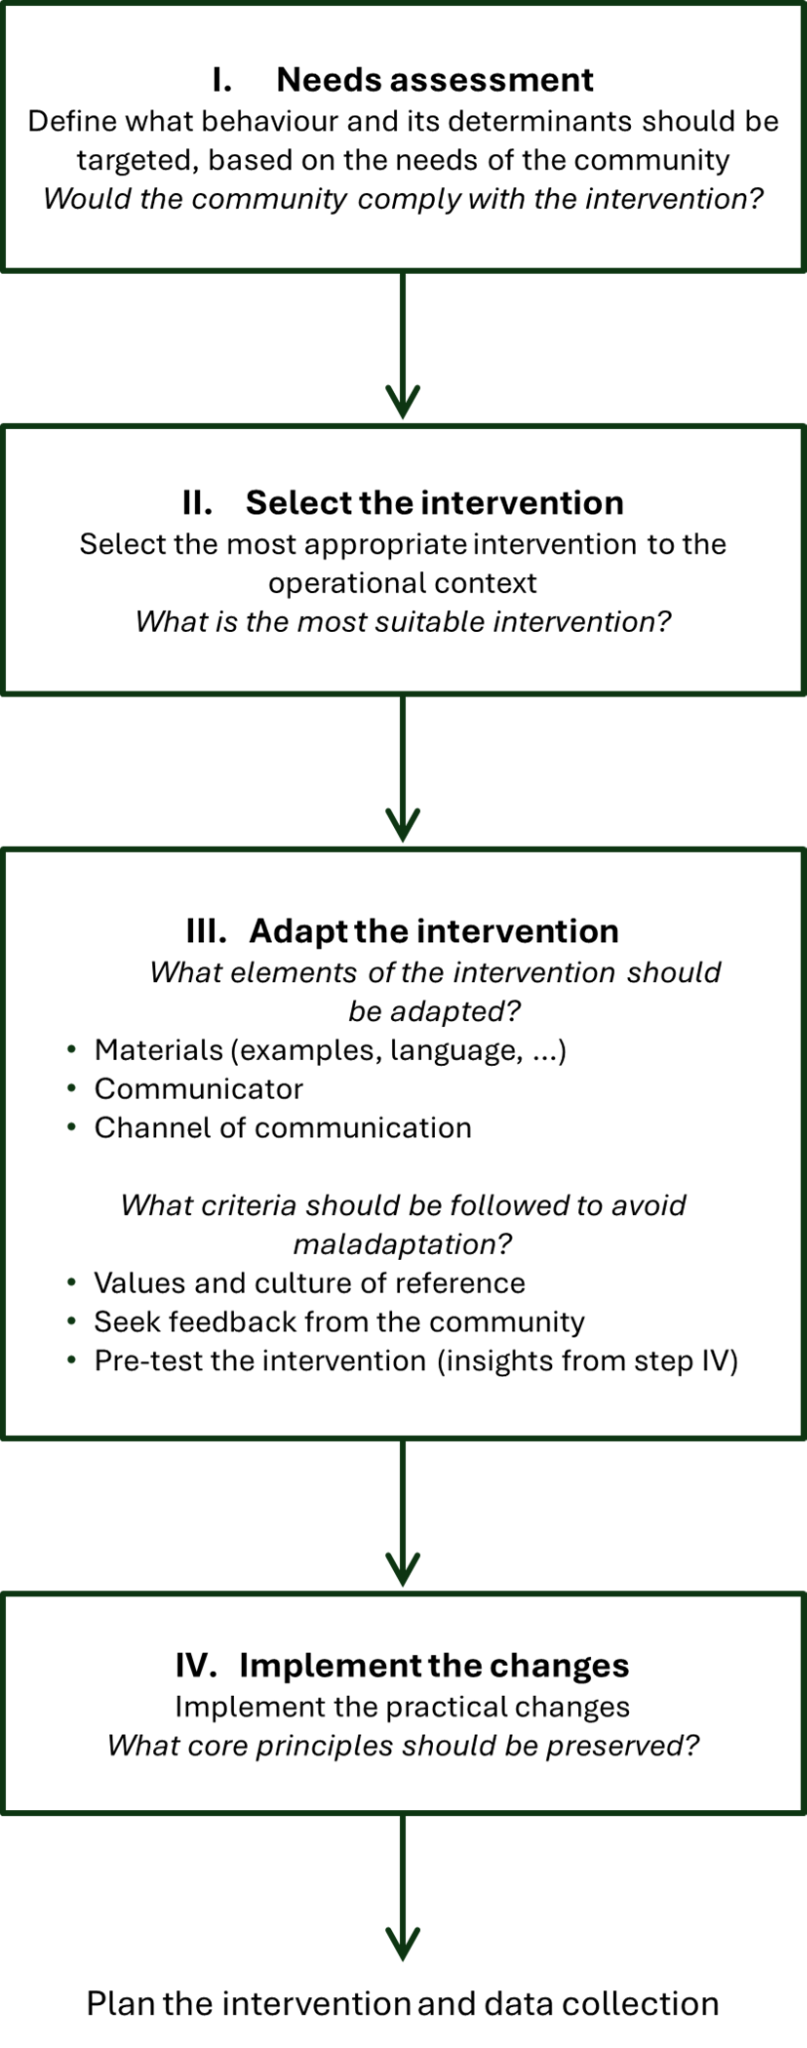
\includegraphics[width=\linewidth]{media/image1.png}

		\caption{A flow chart of the adaptation process of evidence-based interventions (EBI) according to Intervention Mapping. Adapted from Highfield et al. (2016).}

		\label{fig:rId8}


	\end{figure}






	The process of adaptation focuses on how to reach the new target group by adjusting components of the intervention so that participants will relate to it in the intended way.\footnote{ Most adapted interventions are developed with reference to a population with certain characteristics (e.g. highly educated, urbanized) and adapted to other contexts. However, the theoretical model approach does not assume this direction, and it is in principle possible to do the opposite, i.e. to adapt interventions that were developed in rural areas or with less educated samples.} Adaptation occurs by assessing the cultural fit of the intervention: how its format, design, and materials will be received in the new context and meet the needs and style of thinking of the community. Evidence on how to conduct this process relies heavily on existing applications, and there is no single guideline (Escoffery et al., 2019). There are however several points in common among the various approaches: the editing of the intervention structure and content, the selection of the delivery channel, seeking feedback, and pre-testing.



	Intervention materials are the first elements of an intervention to be placed under scrutiny. Oftentimes the original examples and depictions need to be updated to reflect the specific problems faced by the community: In the case of misinformation treatments, this could mean adjusting the kind of stimuli to be evaluated, in terms of their focus and rhetoric, but also about who is spreading the message and through what channels. One example is the adaptation process of the inoculation game “Cranky Uncle.” Originally developed for a U.S. audience, the intervention underwent conspicuous modifications to its design and materials for adaptation to East African countries (Hopkins et al., 2023). These changes included a different representation of healthcare workers, localization of expressions and cultural references, and the incorporation of fact-based explanations alongside the original game's logic-based explanations. Values and cultural references also play a role. For instance, appeals to the common good or trust in authorities might be perceived as untrustworthy in countries with strong authoritarian governments. Going back to the above-mentioned digital boundaries, experimenters also need to take into account the level of accessibility of the intervention: For example, researchers have to assess the literacy levels of respondents to adapt the content accordingly (Card et al., 2011), or at least monitor them at the time of data acquisition (Ali \& Qazi, 2023). The use of abstract-logical concepts should also be moderated, following insights from the work on sign development. In summary, adapting the materials and structure of an intervention is not a simple language translation but rather an act of cultural and demographic localization.



	Adaptation also operates through the choice of the delivery channel: Which tools, practices and operators mediate the transmission of the intervention must also be considered in terms of their effectiveness within the new population. We have already speculated how the respondents' unfamiliarity with the devices provided for responding may have contributed to the negative outcome of the study, and that the use of more traditional means of communication may help an intervention penetrate a community (Badrinathan et al., 2024). Human communication is yet another crucial element that can tilt the balance in an intervention. When interventions are conducted door-to-door, it is not trivial to determine who is the most suitable person to perform such a task. On the one hand, university staff may be the most authoritative, and their expertise may help increase compliance with and attentiveness towards the intervention. On the other hand, members of the same community may be able to understand and navigate the nuances of the given context and appear more trustworthy, potentially reaching more respondents.



	When adapting both the delivery channels and the structure and content of the intervention, it is worth seeking relevant feedback from members of the community. These conversations might reveal important and previously unaccounted-for information, such as the presence of particular risk or protective factors. This point is also made by Harjani and colleagues in the discussion when they suggest that the study would have benefited from “stronger local relationships as well as a greater accountability of the diversity within countries” (Harjani et al., 2023, p. 12). The idea of involving relevant stakeholders in the decision-making process also has a long history in clinical research, exemplified by the concept of co-design (see, for instance, Robert, 2013). In misinformation research, a risk factor might be represented by the channels through which false information is spread, which might be difficult to reach directly or replicate due to technical or language barriers. Conversely, a protective factor might be the presence of influential community leaders who are willing to collaborate in the field.



	Lastly, a common feature of adaptation strategies is the pre-testing of the intervention. When all potential adaptations have been defined on paper, it is essential to conduct pilot tests whenever possible to determine whether changes are effectively reducing the foreseen obstacles or if finer tuning is needed. The resulting process of trial and error, familiar to readers of this journal, is time-consuming and resource-intensive, but often essential to the development of applied interventions.



	\section{Conclusions and Future Directions}



	The findings of Harjani et al. (2023) underscore the limitations and challenges of applying digital inoculation interventions against misinformation in less urbanized and literate populations. Their study, which focused on rural Indian participants, revealed no significant effects of the adapted inoculation game on misinformation resistance. The authors justifiably highlighted the critical role of both digital and cultural barriers in the effectiveness of such interventions. We have proposed incorporating a cultural-historical perspective into intervention design, as it can provide deeper insights into how stages of conceptual development influence the reception and efficacy of misinformation interventions. Furthermore, we have proposed the application of Intervention Mapping as a systematic method for tailoring interventions to specific cultural contexts. By combining theoretical insights from psychological development with practical guidance inspired by research on the adaptation of medical treatments, we hope to inspire the design of more culturally attuned strategies to fight misinformation. Specifically, researchers should carefully identify the specific characteristics of the population being tested to select and adapt interventions, both in terms of typical reasoning styles and relevant cultural components.



	As is to be expected, our proposal comes with a few caveats. The cultural-historical perspective is an influential theory from the history of psychology. However, even though some of its tenets have seen a resurgence in recent decades, there is still much work to do in further developing these theories and subjecting them to experimental testing. In the same vein, given that these theories are still highly general and theoretical, drawing practical implications is not always straightforward and may require additional leaps of thought that should be tested at each step. Moreover, although Intervention Mapping may represent a promising direction to help guide adaptation of interventions, this field originated only recently and is continuously evolving. Therefore, our guidelines are accompanied by a series of caveats. First, deviations from the original protocols are inherently risky, as Harjani and colleagues also suggest: Some interventions may show greater effectiveness when they preserve their original form. With too much focus on cultural fitting, there is indeed a risk of adaptation “hyperactivity” that may reduce rather than increase the fit of the intervention (Evans et al., 2021). Second, adaptations can be burdensome: Strengthening an intervention may require an investment of resources that is not always possible. Last, the recency of theories such as Intervention Mapping and the cultural variability of different settings entails that there is a lack of uniform evidence about which adaptations are most effective. There is much to be learned about this process, but also several opportunities to put it to a test.



	As a final remark, we hasten to note that different ways exist to adapt an intervention to its context (i.e., target population, environment, and target outcome). In the present paper, we mainly focus on a top-down approach to the adaptation of inoculation interventions online, namely, starting from interventions that were already developed for a specific population and adapting these to another population. An alternative, bottom-up approach to develop an adaptive intervention is to create a contextualized, that is, population-specific, intervention in close cooperation with representatives of this specific population. In this case, the resulting intervention is not a practical adaptation of an existing intervention but implements the features of the underlying theory for the intervention (here e.g., inoculation theory), in accordance with feedback from the population of interest. While the former (adapting existing interventions) is usually more resource efficient, the latter (creating an intervention from scratch) has the potential for high effectiveness by a maximized fit between the intervention and the focused population. We also do not intend to imply that interventions for rural societies are merely simplified versions of Western approaches. However, interventions relying heavily on formal logic, which often require formal schooling, may be less effective in rural societies where access to such education is limited. Interventions designed for contexts where everyday concepts dominate should account for this, alongside other population characteristics. Future research should therefore be conducted combining theoretical insights from cultural-historical psychology and Intervention Mapping to empirically test the effectiveness of mis- and disinformation interventions in different cultural contexts. For example, one could imagine a study that first investigates the dominant method of thinking (i.e., everyday versus logical concepts) in two given populations and subsequently applies an inoculation intervention and an alternative intervention in both populations. If our theory proves to be correct, the inoculation intervention should prove to be more effective in the population where thinking with logical concepts is dominant compared to the population where thinking with everyday concepts is dominant. Similarly, the alternative intervention should be more effective in the population where thinking with everyday concepts is dominant. If our theory is proven correct, interventions can be further developed to specifically target different types of populations, thereby contributing to the global fight against mis- and disinformation.











	\section{References}



	Alderson-Day, B. \& Fernyhough, C. (2015). Inner speech: Development, cognitive functions, phenomenology, and neurobiology. \emph{Psychological Bulletin}, \emph{141}(5), 931-965. \url{https://doi.org/10.1037/bul0000021}



	Ali, A. \& Qazi, I. A. (2023). Countering misinformation on social media through educational interventions: Evidence from a randomized experiment in Pakistan. \emph{Journal of Development Economics, 163}, Article 103108. \url{https://doi.org/10.1016/j.jdeveco.2023.103108}



	Amar, P., Badrinathan, S., Chauchard F., \& Sichart, F. (2024). Countering misinformation early: Evidence from a classroom-based field experiment in India [Unpublished manuscript]. \url{https://priyadarshiamar.github.io/Assets/Mercury\_SSRC.pdf}



	Ardila, A., Bertolucci, P. H., Braga, L. W., Castro-Caldas, A., Judd, T., Kosmidis, M. H., Matute, E., Nitrini, R., Ostrosky-Solis, F., \& Rosselli, M. (2010). Illiteracy: The neuropsychology of cognition without reading. \emph{Archives of Clinical Neuropsychology : The Official Journal of the National Academy of Neuropsychologists}, \emph{25}(8), 689--712. \url{https://doi.org/10.1093/arclin/acq079}



	Ardila, A., \& Rosselli, M. (2007). Illiterates and cognition: The impact of education. In B. Uzzell, M. Pontón, A. Ardilla (Eds.)., \emph{International handbook of cross-cultural neuropsychology }(pp. 191-208). Lawrence Erlbaum Associates.



	Arechar, A. A., Allen, J., Berinsky, A. J., Cole, R., Epstein, Z., Garimella, K., Gully, A., Lu, J. G., Ross, R. M., Stagnaro, M. N., Zhang, Y., Pennycook, G., \& Rand, D. G. (2023). Understanding and combatting misinformation across 16 countries on six continents. \emph{Nature Human Behaviour, 7}, 1502-1513. \url{https://doi.org/10.1038/s41562-023-01641-6}



	Athey, S., Cersosimo, M., Koutout, K., \& Li, Z. (2022). Emotion- versus reasoning-based drivers of misinformation sharing: A field experiment using text message courses in Kenya. \emph{Working Paper.} \url{https://www.gsb.stanford.edu/faculty-research/working-papers/emotion-versus-reasoning-based-drivers-misinformation-sharing-field}



	Badrinathan, S. (2021). Educative interventions to combat misinformation: Evidence from a field experiment in India. \emph{American Political Science Review, 115}(4), 1325-1341. \url{https://doi.org/10.1017/S0003055421000459}



	Badrinathan, S., Chauchard, S., \& Siddiqui, N. (2024). Misinformation and support for vigilantism: An experiment in India and Pakistan. \emph{American Political Science Review}. 1--19. \url{https://doi.org/10.1017/S0003055424000790}



	Badrinathan, S., \& Chauchard, S. (2024). Researching and countering misinformation in the Global South. \emph{Current Opinion in Psychology, 55}, Article 101733. \url{https://doi.org/10.1016/j.copsyc.2023.101733}



	Highfield L., Hartman M., Mullen P. D., \& Leerlooijer J. N. (2016). Chapter 10: Using intervention mapping to adapt evidence-based interventions. In L. K. Bartholomew Eldredge, C. M. Markham, R. A. C. Ruiter, M. E. Fernandez, G. Kok, G. S. Parcel (Eds.), \emph{Planning health promotion programs: An intervention mapping approach} (pp. 597--649). Jossey-Bass.



	Basol, M., Roozenbeek, J., \& van der Linden, S. (2020). Good news about bad news: Gamified inoculation boosts confidence and cognitive immunity against fake news. \emph{Journal of Cognition, 3}(1), Article 2. \url{https://doi.org/10.5334/joc.91}



	Blair, R. A., Gottlieb, J., Nyhan, B., Paler, L., Argote, P., \& Stainfield, C. J. (2023). Interventions to counter misinformation: Lessons from the Global North and applications to the Global South. \emph{Current Opinion in Psychology, 55}, Article 101732. \url{https://doi.org/10.1016/j.copsyc.2023.101732}



	Brown, E. K. (Ed.). (2005). \emph{Encyclopedia of language \& linguistics} (2nd Edition). Elsevier.



	Bowles, J., Croke, K., Larreguy, H., Marshall, J., \& Liu, S. (2023). Sustaining exposure to fact-checks: Misinformation discernment, media consumption, and its political implications. \emph{SSRN.} \url{https://doi.org/10.2139/ssrn.4582703}



	Bowles, J., Larreguy, H., \& Liu, S. (2020). Countering misinformation via WhatsApp: Preliminary evidence from the COVID-19 pandemic in Zimbabwe. \emph{PloS One, 15}(10), Article e0240005. \url{https://doi.org/10.1371/journal.pone.0240005}



	Camminga, T. F., Hermans, D., Segers, E., \& Vissers, C. (2024). How word meaning structure relates to executive functioning and theory of mind in children with developmental language disorder: A multiple case study. \emph{Autism \& Developmental Language Impairments, 9}, Article 23969415241268245. \url{https://doi.org/10.1177/23969415241268245}



	Card, J. J., Solomon, J., \& Cunningham, S. D. (2011). How to adapt effective programs for use in new contexts. \emph{Health Promotion Practice, 12}(1), 25-35. \url{https://doi.org/10.1177/1524839909348592}



	Dahdouh-Guebas, F., Ahimbisibwe, J., Van Moll, R., \& Koedam, N. (2003). Neo-colonial science by the most industrialised upon the least developed countries in peer-reviewed publishing. \emph{Scientometrics, 56}, 329-343. \url{https://doi.org/10.1023/A:1022374703178}



	Escoffery, C., Lebow-Skelley, E., Udelson, H., Böing, E. A., Wood, R., Fernandez, M. E., \& Mullen, P. D. (2019). A scoping study of frameworks for adapting public health evidence-based interventions. \emph{Translational Behavioral Medicine, 9}(1), 1-10. \url{https://doi.org/10.1093/tbm/ibx067}



	Evans, R. E., Moore, G., Movsisyan, A., \& Rehfuess, E., The ADAPT Panel. (2021). How can we adapt complex population health interventions for new contexts? Progressing debates and research priorities. \emph{Journal of Epidemiology and Community Health, 75}(1), 40-45. \url{https://doi.org/10.1136/jech-2020-214468}



	Gantayat, N., Ashok, A., Manchi, P., Pierce-Messick, R., Porwal, R., \& Gangaramany, A. (2024). Taking the big leap | understanding, accessing and improving behavioural science interventions. \emph{Frontiers in Public Health}, \emph{12}, Article 1355539. \url{https://doi.org/10.3389/fpubh.2024.1355539}



	Garg, N., \& Yadav, M. (2022). Learning to Resist Misinformation. \emph{Working Paper.} \url{https://assets.namangarg.net/papers/jmp\_latest.pdf}



	Gavin, L., McChesney, J., Tong, A., Sherlock, J., Foster, L., \& Tomsa, S. (2022). Fighting the spread of COVID-19 misinformation in Kyrgyzstan, India, and the United States: How replicable are accuracy nudge interventions? \emph{Technology, Mind, and Behavior, 3}(3), 1-12. \url{https://doi.org/10.1037/tmb0000086}



	Ghai, S. (2021). It's time to reimagine sample diversity and retire the WEIRD dichotomy. \emph{Nature Human Behaviour 5}, 971--972. \url{https://doi.org/10.1038/s41562-021-01175-9}



	Guess, A. M., Lerner, M., Lyons, B., Montgomery, J. M., Nyhan, B., Reifler, J., \& Sircar, N. (2020). A digital media literacy intervention increases discernment between mainstream and false news in the United States and India. \emph{Proceedings of the National Academy of Sciences}, \emph{117}(27), 15536-15545. \url{https://doi.org/10.1073/pnas.1920498117}



	Guess, A. M., \& Munger, K. (2022). Digital literacy and online political behavior. \emph{Political Science Research and Methods, 11}(1), 110-128. \url{https://doi.org/10.1017/psrm.2022.17}



	Gottlieb, J., Adida, C. L., \& Moussa, R. (2022). Reducing misinformation in a polarized context: Experimental evidence from Côte d'Ivoire. \emph{Working Paper.} \url{https://doi.org/10.26085/C3Q30T}



	Henrich, J., Heine, S. J., \& Norenzayan, A. (2010). The weirdest people in the world? \emph{Behavioral and Brain Sciences}, \emph{33}(2-3), 61-83. \url{https://doi.org/10.1017/S0140525X0999152X}



	Hopkins, K. L., Lepage, C., Cook, W., Thomson, A., Abeyesekera, S., Knobler, S., Boehman, N., Thompson, B., Waiswa, P., Nambi Ssanyu, J., Kabwijamu, L., Wamalwa, B., Aura, C., Rukundo, J.C., \& Cook, J. (2023). Co-designing a mobile-based game to improve misinformation resistance and vaccine knowledge in Uganda, Kenya, and Rwanda. \emph{Journal of Health Communication}, \emph{28}(sup2), 49--60. \url{https://doi.org/10.1080/10810730.2023.2231377}



	Horta Ribeiro, M., Cheng, J., \& West, R. (2023). Automated content moderation increases adherence to community guidelines. \emph{Proceedings of the ACM Web Conference 2023,} 2666-2676. \url{https://doi.org/10.1145/3543507.3583275}



	Hruschka, D. J., Munira, S., Jesmin, K., Hackman, J., \& Tiokhin, L. (2018). Learning from failures of protocol in cross-cultural research. \emph{Proceedings of the National Academy of Sciences}, \emph{115}(45), 11428-11434. \url{https://doi.org/10.1073/pnas.1721166115}



	Iyengar, A., Gupta, P., \& Priya, N. (2023). Inoculation against conspiracy theories: A consumer side approach to India's fake news problem. \emph{Applied Cognitive Psychology}, \emph{37}(2), 290-303. \url{https://doi.org/10.1002/acp.3995}



	Katsaros, M., Grüning, D. J., \& Lou, S. (2024). Offensive comment filtering impact on online engagement: A large-scale randomized controlled trial on Nextdoor. \emph{PsyArXiv.} \url{https://doi.org/10.31234/osf.io/nxuqy}



	Kiili, K., Siuko, J., \& Ninaus, M. (2024). Tackling misinformation with games: A systematic literature review. \emph{Interactive Learning Environments}, \emph{32}(10), 7086-7101. \url{https://doi.org/10.1080/10494820.2023.2299999}



	Lin, H., Garro, H., Wernerfelt, N., Shore, J. C., Hughes, A., Deisenroth, D., Barr, N., Berinsky, A. J., Eckles, D., Pennycook, G., \& Rand, D. G. (2024). Reducing misinformation sharing at scale using digital accuracy prompt ads. \emph{PsyArXiv.} \url{https://doi.org/10.31234/osf.io/u8anb}



	Luria, A. R. (1976). \emph{Cognitive Development: Its Cultural and Social Foundations }(M. Lopez-Morillas \& L. Solotaroff, Trans.). Harvard University Press.



	Ma, J., Chen, Y., Zhu, H., Gan, Y. (2023). Fighting COVID-19 misinformation through an online game based on the inoculation theory: Analyzing the mediating effects of perceived threat and persuasion knowledge. \emph{International Journal of Environmental Research and Public Health, 20}(2), 980. \url{https://doi.org/10.3390/ijerph20020980}



	Matias, J. N. (2019). Preventing harassment and increasing group participation through social norms in 2,190 online science discussions. \emph{Proceedings of the National Academy of Sciences}, \emph{116}(20), 9785-9789. \url{https://doi.org/10.1073/pnas.1813486116}



	McGuire, W. J. (1961). Resistance to persuasion conferred by active and passive prior refutation of the same and alternative counterarguments. \emph{The Journal of Abnormal and Social Psychology}, 63(2), 326--332. \url{https://doi.org/10.1037/h0048344.}



	Mothkoor, V., \& Mumtaz, F. (2021). The digital dream: Upskilling India for the future. \emph{Ideas for India. \url{https://www.ideasforindia.in/topics/governance/the-digital-dream-upskilling-india-for-the-future.html}}



	Offer-Westort, M., Rosenzweig, L.R. \& Athey, S. (2024). Battling the coronavirus ‘infodemic' among social media users in Kenya and Nigeria. \emph{Nature Human Behaviour}, \emph{8}, 823--834. \url{https://doi.org/10.1038/s41562-023-01810-7}



	Pereira, F. B., Bueno, N. S., Nunes, F., \& Pavão, N. (2022). Inoculation reduces misinformation: Experimental evidence from multidimensional interventions in Brazil. \emph{Journal of Experimental Political Science}, \emph{11}(3), 239-250. \url{https://doi.org/10.1017/XPS.2023.11}



	Porter, E., \& Wood, T. J. (2021). The global effectiveness of fact-checking: Evidence from simultaneous experiments in Argentina, Nigeria, South Africa, and the United Kingdom. \emph{Proceedings of the National Academy of Sciences}, \emph{118}(37), Article e2104235118. \url{https://doi.org/10.1073/pnas.2104235118}



	Porter, E., Velez, Y., \& Wood, T. J. (2023). Correcting COVID-19 vaccine misinformation in 10 countries. \emph{Royal Society Open Science}, 10(3), Article 221097. \url{https://doi.org/10.1098/rsos.221097}



	Registrar General of India. (2011). \emph{Census of India 2011}. www.censusindia.gov.in



	Robert, G. (2013). Participatory action research: Using experience-based co-design to improve the quality of healthcare services. In S. Ziebland, J. Calabrase, A. Coulter, \& L. Locock (Eds.) \emph{Understanding and Using Experiences of Health and Illness }(pp. 138-149)\emph{.}. Oxford University Press. \url{https://doi.org/10.1093/acprof:oso/9780199665372.003.0014}



	Roozenbeek, J., van der Linden, S., Goldberg, B., Rathje, S., \& Lewandowsky, S. (2022). Psychological inoculation improves resilience against misinformation on social media. \emph{Science Advances}, \emph{8}(34), Article eabo6254. \url{https://doi.org/10.1126/sciadv.abo6254}



	Roozenbeek, J., Remshard, M., \& Kyrychenko, Y. (2024). Beyond the headlines: On the efficacy and effectiveness of misinformation interventions. \emph{advances.in/psychology}, 2, Article e24569. \url{https://doi.org/10.56296/aip00019}



	Saxena, K., \& John, N. (2021, December 3). Mind your language: How fake news is clean-bowling big tech and what needs to be done. \emph{The Economic Times}. \url{https://economictimes.indiatimes.com/prime/technology-and-startups/mind-your-language-how-fake-news-is-clean-bowling-big-tech-and-what-needs-to-be-done/primearticleshow/88058557.cms?from=mdr}



	Toomela, A. (2005). Decision making with incomplete information: Systemic and nonsystemic ways of thinking in psychology and medicine. In R. Bibace, J. D. Laird, K. L. Noller \& J. Valsiner (Eds.), \emph{Science and medicine in dialogue: Thinking through particulars and universals} (pp. 231-241). Greenwood Publishing. \url{https://psycnet.apa.org/record/2005-01866-014.}



	Toomela, A. (2020a). \emph{Culture, speech, and My Self. }Porcos ante Margaritas.



	Toomela, A. (2020b). Studies in the mentality of literates: Searching for the cultural Great Divide at the individual level of analysis. \emph{Integrative Psychological and Behavioral Science}, \emph{54}, 1-29. \url{https://doi.org/10.1007/s12124-019-09503-5}



	Toomela, A., Filho, D. B., Bastos, A. C. S., Chaves, A. M., Ristum, M., Chaves, S. S., \& Salomão, S. J. (2020a). Studies in the mentality of literates: 2. Conceptual structure, cognitive inhibition and verbal regulation of behavior. \emph{Integrative Psychological and Behavioural Science}, \emph{54}, 880--902. \url{https://doi.org/10.1007/s12124-020-09517-4}



	Toomela, A., Filho, D. B., Bastos, A. C. S., Chaves, A. M., Ristum, M., Chaves, S. S., \& Salomão, S. J. (2020b). Studies in the mentality of literates: 1. Conceptual structure and aspects of visual perception. \emph{Integrative Psychological and Behavioral Science}, \emph{54}, 465-493. \url{https://doi.org/10.1007/s12124-019-09511-5}



	Toomela, A., Filho, D. B., Bastos, A. C. S., Chaves, A. M., Ristum, M., Chaves, S. S., Salomão, S. J., \& Pulver, A. (2023). Studies in the mentality of literates: 3. Conceptual structure and nonsense of personality testing. \emph{Integrative Psychological and Behavioral Science}, \emph{57}, 117-150. \url{https://doi.org/10.1007/s12124-022-09706-3}



	Translators without Borders. (2019). \emph{Language data for Nigeria}. \url{https://translatorswithoutborders.org/northeast-nigeria-language-map/}



	Valsiner, J., Chaudhary, N., \& Benetka, G. (2017). \emph{From methodology to methods in human psychology}. Springer International Publishing. SpringerBriefs in Psychology. \url{https://doi.org/10.1007/978-3-319-61064-1}



	Van der Linden, S. (2023). Psychological inoculation against misinformation. \emph{Journal of Neurology, Neurosurgery \& Psychiatry, 94}(12), Article e2. \url{https://doi.org/10.1136/JNNP-2023-BNPA.9}



	Vygotsky, L.S. (2012). \emph{Thought and language. }(E. Hanfmann \& G. Vakar, Trans.) MIT Press. (Original work published 1934).


\end{document}